\usetikzlibrary{arrows.meta}
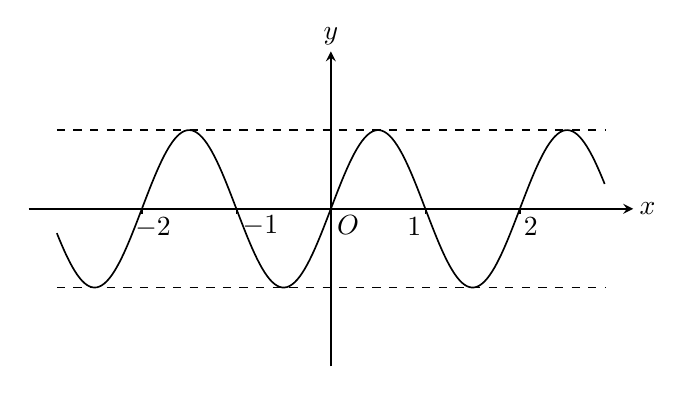
\begin{tikzpicture}[x=1.2cm,y=1.0cm,line width=.6pt,>=stealth,font=\normalsize]
\draw[->] (-3.1999999999999997,0)--(3.1999999999999997,0) node[right,inner sep=0pt,xshift=2pt] {$x$};
\draw[->] (0,-2.0)--(0,2.0) node[above,inner sep=0pt,yshift=2pt] {$y$};
\draw (-2,0)--(-2,-0.07);
\draw (-1,0)--(-1,-0.07);
\draw (1,0)--(1,-0.07);
\draw (2,0)--(2,-0.07);
\node[below,inner sep=0pt,xshift=4pt,yshift=-3pt] at (-2,0) {$-2$};
\node[below right,inner sep=0pt,xshift=2pt,yshift=-2pt] at (-1,0) {$-1$};
\node[below,inner sep=0pt,xshift=-4pt,yshift=-3pt] at (1,0) {$1$};
\node[below,inner sep=0pt,xshift=4pt,yshift=-3pt] at (2,0) {$2$};
\node[below right,inner sep=0pt,xshift=2pt,yshift=-2pt] at (0,0) {$O$};
\draw[dashed] (-2.9,1)--(2.9,1);
\draw[dashed] (-2.9,-1)--(2.9,-1);
\draw[domain=-2.9:2.9,samples=220] plot (\x,{sin(deg(pi*\x))});
\end{tikzpicture}
